\subsection{Lawn Mower Benchmark}
Here we describe dynamics of a lawn mower as introduced in \cite{foldager2017development}. A conceptual model of the driverless lawn mower is shown in Fig. \ref{subfig1}. The lawn mower is steered by controlling the velocity separately on the two driving wheels. A sketch of the vehicle is shown in Fig. \ref{subfig2} and its chassis and caster wheels are shown in Fig. \ref{subfig3}.
\begin{figure}[hpt]
\centering
\subfigure[]{\includegraphics[scale=0.26]{figures/Lawn_Mower.png}\label{subfig1}}
\subfigure[]{\includegraphics[scale=0.19]{figures/fig1.png}\label{subfig2}}
\subfigure[]{\includegraphics[scale=0.19]{figures/fig2_1.png}\label{subfig3}}
\caption{Lawn mower schematics \cite{foldager2017development}}
\label{Lawn_Mower}
\end{figure}

\subsubsection{Dynamical model}
The dynamic response of the lawn mower can be described by the following 6-dimensional nonlinear stochastic differential equation
\begin{align}
\dot{x}_1 &= \frac{1}{I_{zz}}\left ( A_{fy}\sin\Big ( x_6+\frac{\pi}{2}\Big )a+2C_{\gamma}\tan\Big ( \frac{2(x_2-bx_1)}{(V_r+V_l)}\Big )b \right ),\nonumber\\
\dot{x}_2 &= \frac{1}{M}\left ( A_{fy}\sin\Big ( x_6+\frac{\pi}{2}\Big )-2C_{\gamma}\tan\Big(  \frac{2(x_2-bx_1)}{(V_r+V_l)}\Big )\right )- \frac{V_r+V_l}{2}x_1,\nonumber\\
\dot{x}_3 &= \frac{V_r+V_l}{2}\cos(x_5),\\
\dot{x}_4 &= \frac{V_r+V_l}{2}\sin(x_5),\nonumber\\
\dot{x}_5 &= \frac{V_r-V_l}{2D}+x_1+w_{d1},\nonumber\\
\dot{x}_6 &= -\frac{V_r+V_l}{2d}\cos(x_6)-\frac{(V_r-V_l)(d+\sqrt{D^2+(a+b)^2}\sin(x_6))}{2Dd}+w_{d2},\nonumber
\end{align}
where $x_1$, $x_2$, $x_3$, $x_4$, $x_5$, and $x_6$ are respectively yaw, yaw rate, $x$, $y$, angle of vehicle with respect to $x$-axis ($\theta$), and relative orientation of caster wheel ($\beta$), respectively. The $w_{d1}$ and $w_{d2}$ are noises in orientation and angle of caster wheel generated due to uneven ground surface. $V_r$ and $V_l$ are the control inputs representing velocity of right and left driving wheels, respectively.
%Fig.~\ref{Lawn_Mower} shows the schematic of lawn mower.
The remaining parameters are listed in Table~\ref{table_parameter}.
% Please add the following required packages to your document preamble:
% \usepackage{booktabs}
\begin{table}[]
\centering
\caption{Lawn mower parameters}
\label{table_parameter}
\begin{tabular}{@{}ll@{}}
\toprule
Mass, M                      & 700$kg$                     \\
Axle half width, D                & 1.2$m$                      \\
Dimensions, (a, b)           & 1.35$m$, 0.15$m$                \\
Caster wheel offset, d       & 0.1$m$                        \\
$A_{fy}$                    & 199                         \\
$I_{zz}$                    & 394 $Kg$-$m^2$ \\
$C_{\gamma}$ & 22000                       \\ \bottomrule
\end{tabular}
\end{table}

It is possible to extend the dynamics by modelling the response of the steering mechanism using a first order equation for each driving wheel:
\begin{align*}
\dot{V_l} = -k_\tau\cdot (V_l - V_l^{sp}),\\
\dot{V_r} = -k_\tau\cdot (V_r - V_r^{sp}),
\end{align*}
where $V_l^{sp}$ and $V_r^{sp}$ are velocity set points specified by the controller, and $k_\tau$ is a gain determined experimentally.
In the following, we assume that velocities $V_l$ and $V_r$ can be directly specified by the controller. In other words, $k_\tau$ is very large in compare with the sampling time of the controller and $V_l(t)\approx V_l^{sp}$ and $V_r(t) \approx V_r^{sp}$.

\subsubsection{Controller mechanism}
The main objective for the lawn mower is to cover a given area as soon as it can. This can be seen as a path planning problem and is usually achieved by specifying a set of way-points, and the task of the controller would be to move from an initial position in the vicinity of the current way-point to the vicinity of the next way-point.
%\noindent
%\textbf{Controller 1.}
We provide simple On-Off type controller for lawn mover to reach desired position $(x_d,y_d)$. Consider base velocity $V_b$ and boost velocity $V_d$.  
 The control inputs that is velocities of right and left wheel are given as
\begin{align}
V_r&=V_b+V_d \text{sgn}(\sin(\theta_d-x_5))\nonumber\\
V_l&=V_b-V_d \text{sgn}(\sin(\theta_d-x_5)),\label{eq:controller}
\end{align}
where $\theta_d=\text{atan2}((y_d-x_4),(x_d-x_3))$.
The closed-loop response starting from initial condition $[0,0,0,0,0]^T$ reaching desired location $(x_d,y_d)=(-10,-5)$ with selection of $V_b=2$ and $V_d=1.5$ is shown in Fig.~\ref{fig3}.
\begin{figure}[hpt]
\centering
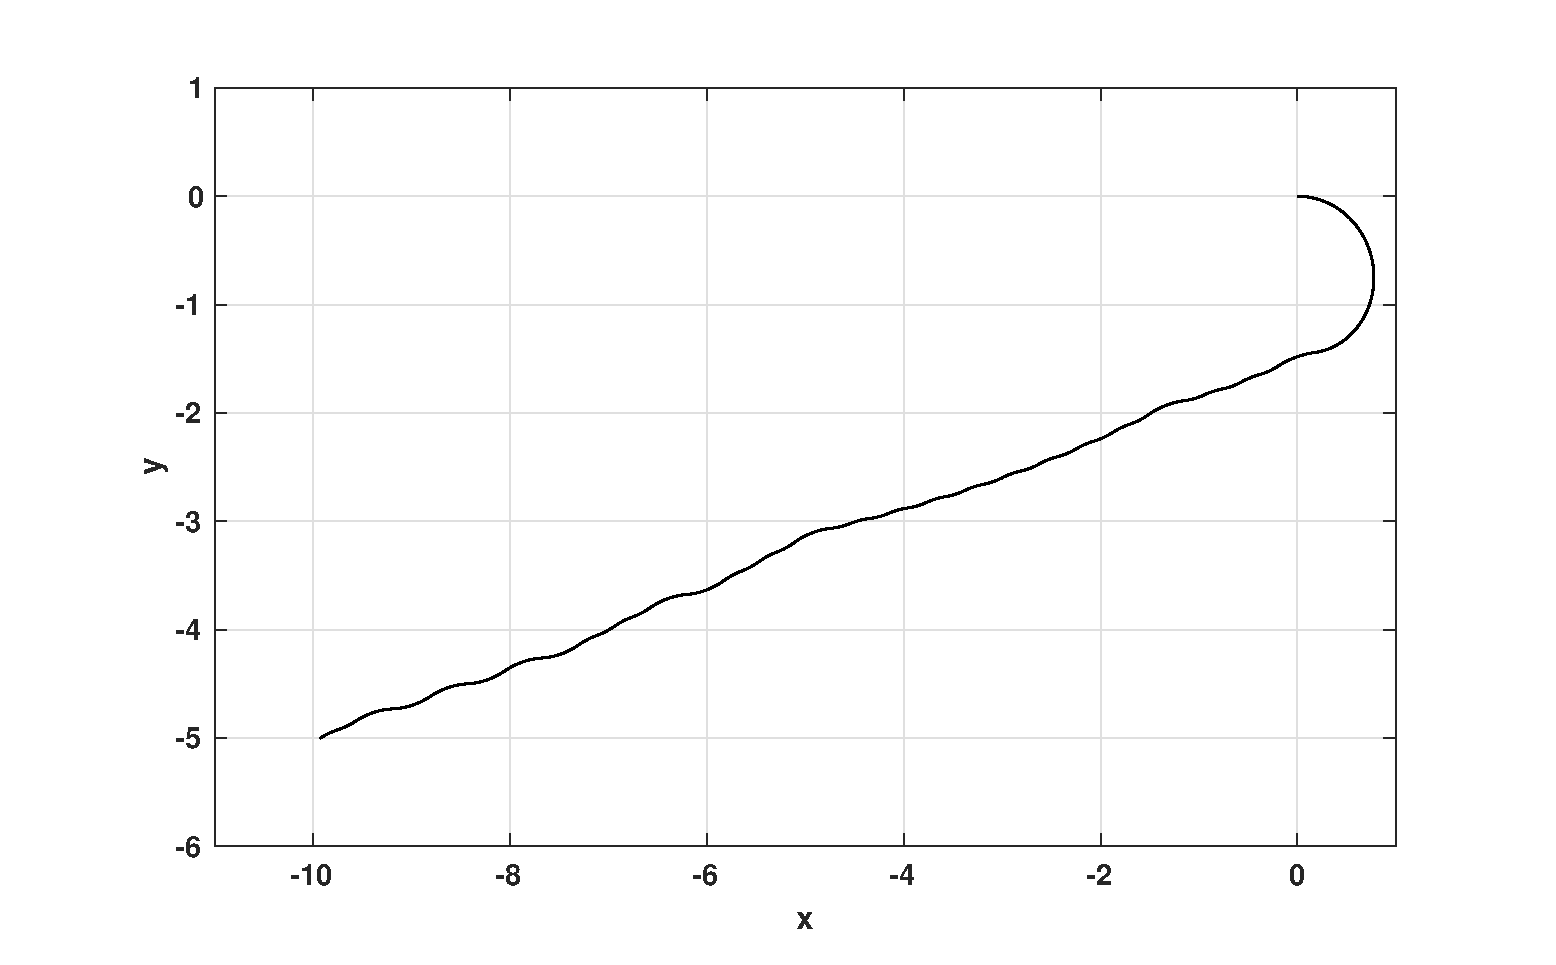
\includegraphics[scale=0.8,height=5cm]{figures/resp1}
\caption{Closed-loop response of lawn mower}
\label{fig3}
\end{figure}

% \noindent
% \textbf{Controller 2.}
% We provide PI controller for lawn mover to reach desired position $(x_d,y_d)$. Consider base velocity $V_b$, and $u_1$ and $u_2$ as a boost velocity for right and left wheels, respectively. The velocity of right and left wheel is given as
% \begin{align*}
% V_r&=V_b+u_1,\\
% V_l&=V_b+u_2.
% \end{align*}
% The error in current position and desired position is given by $e_p=\sqrt{(x_d-x_3)^2+(y_d-x_4)^2}$ and is used to calculate base velocity as $V_b=k_p e_p$, where $k_p>0$ is a proportional gain. For computing $u_1$ and 
% $u_2$, we need misalignment between the orientation of vehicle and orientation of desired position, and it is calculated as
% \[\theta_e=\text{atan2}(\sin(\theta_d-x_5),\cos(\theta_d-x_5)),\]
% where $\theta_d=\text{atan2}((y_d-x_4),(x_d-x_3))$. The $u_1$ and $u_2$ are computed as
% \begin{align*}
% \begin{matrix}
% \begin{bmatrix}
% u_1\\ 
% u_2
% \end{bmatrix}=\begin{bmatrix}k\theta_e+k_i\int \theta_e\\ 
% 0
% \end{bmatrix}, & \text{if } \theta_e>0,
% \\
% \begin{bmatrix}
% u_1\\ 
% u_2
% \end{bmatrix}=\begin{bmatrix}0\\ 
% k\theta_e+k_i\int \theta_e
% \end{bmatrix}, & \text{if } \theta_e<0,
% \end{matrix}
% \end{align*}  
% where $k,k_i>0$ are proportional and integral gains. The trajectory starting from initial condition $[0,0,0,0,0]^T$ reaching desired location $(x_d,y_d)=(-10,-5)$ is shown in Figure \ref{fig2}.
% \begin{figure}[hpt]
% \centering
% 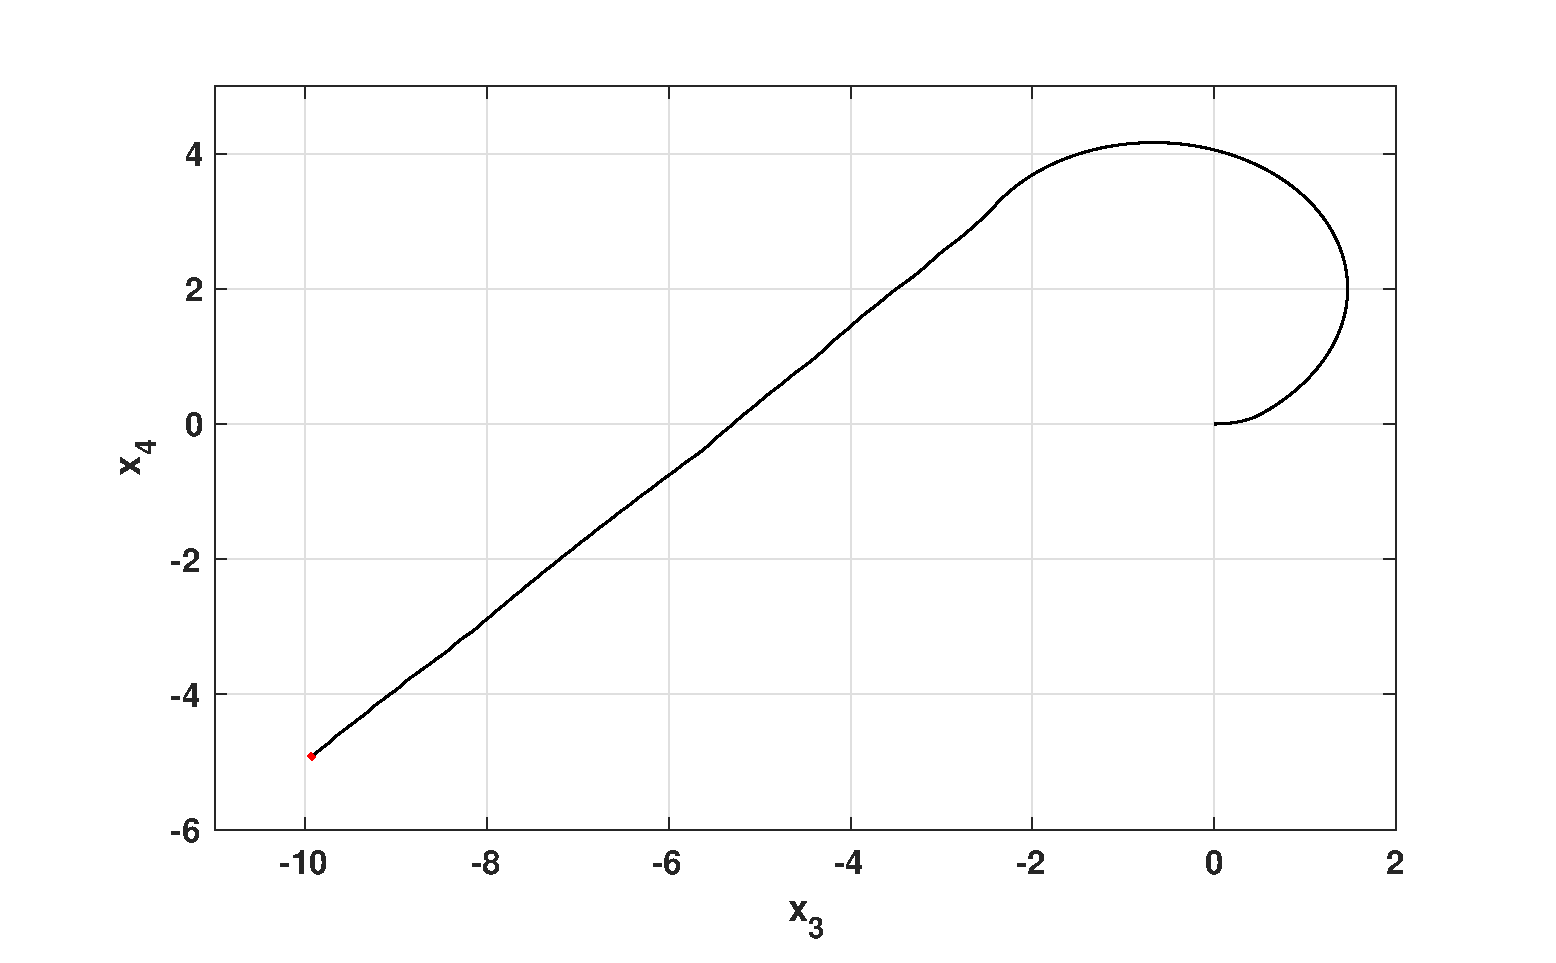
\includegraphics[scale=0.8,height=5cm]{figures/resp}
% \caption{Closed-loop response of lawn mower}
% \label{fig2}
% \end{figure} 

\subsubsection{Specification of interest}
% Therefore, the first interesting problem will be to find probability of reaching a target set while avoiding hitting boundaries of the area.
%\begin{equation*}
%\mathbb P()
%\end{equation*}
The controller of the previous subsection does not take into account avoiding obstacles and preventing collision with boundaries of the area. Here we define a specification that computes probability of avoiding obstacles over finite-time traces of the system. 

The state space of the system is $X=\mathbb R^{6}$. We consider the region $X_0 = [-0.5,0.5]^2\times[-1,1]^2\times[-\pi,\pi]^2$ for the initial state of the system and $X_1 = [-0.5,0.5]^2\times[-4,4]\times[2.5,4]\times[-\pi,\pi]^2$ for the obstacles or one of the boundaries of the area. The set of atomic propositions is given by $\Pi=\{p_0,p_1,p_2\}$ with labeling function $L(x_i) = p_i$ for all $x_i\in X_i$, $i\in\{0,1,2\}$, with $X_2 := X\backslash (X_0\cup X_1)$ . The objective is to compute a lower bound $\alpha>0$ on the probability that the solution process of length $N=200$ satisfies the safe LTL$_f$ formula $p_0\wedge\square^{\le 200}\neg p_1$:
$$\Phi:=\mathbb P_{\ge \alpha}[p_0\wedge\square^{\le 200}\neg p_1].$$

% The next rather complicated problem would be to design a control strategy for fully covering the area using a set of way-points and then ask for the probability of full covering as a function of time.
% Here we tackle the reachability problem.

%\subsection{Reachability Probability}

